\documentclass[12pt, letterpaper]{article}
\usepackage[margin=2.4cm]{geometry} % reduced from 2.5 cm to fit table 1 nicely
\usepackage{times}
\usepackage{graphicx}
\usepackage[utf8]{inputenc}
\usepackage[T1]{fontenc}
\usepackage{lmodern}
\usepackage[table,xcdraw]{xcolor}
\usepackage{booktabs}
%%%%%%%%%%%%%%%%%%%%%%%%%%%%%%%%%%%%%%%%%%%%%%%%%%%%
\begin{document}
% title
\fontfamily{ptm}
\title{ENSC 351 - Lab 3: MapReduce\\ \large{- Lab Report -}}
\date{October 17, 2018}
\author{Galen Elfert, Nic Klaassen, Diane Wolf}
\maketitle
% text
\section{Explanation of Workload}
	The workload we designed as a better fit for the MapReduce framework is a distributed merge sort.

\subsection{Conception}
	In the word count implementation, the highly-parallelised map function does virtually no work, and the overhead of spinning up threads and copying the inputs/outputs far outweighs any possible performance benefit.
	Looking for a better workload, we wanted to find an algorithm where a large amount of computation needs to be completed, and that computation can be broken down into discrete parts that can be completed in parallel.
	We also wanted to find an algorithm with a good use for the reduce stage, where some non-trivial amount of work needs to be done combining outputs from the map stage.
	Sorting was chosen as a better alternative to word counts, because it is a somewhat compute-heavy problem that can be easily broken down into chunks that need to be merged together.

	For our distributed merge sort implementation, an array of size $ n $ is broken up into 4 chunks of size $ n/4 $, which are all sorted in parallel in the map stage.
	In the reduce stage, pairs of sorted chunks of the original array are merged into 2 chunks of size $ n/2 $, these 2 merges are also completed in parallel.
	A potential bottleneck in this implementation is the output stage, which must do a final merge of the last 2 chunks of size $ n/2 $.

	In the limit, this algorithm can theoretically achieve a 4x speedup over a traditional merge sort based on equation~\ref{eq:sort}.
	\begin{equation} \label{eq:sort}
	\lim_{n\to\infty} \frac{\frac{n\log{n} - 2n}{4} + \frac{n}{2} + n}{n\log{n}} = \frac{1}{4}
	\end{equation}
	Intuitively, only $O(n)$ work needs to be done sequentially in the 2 merge steps, while the rest of the $O(n\log{n})$ sort is done concurrently on 4 cores.

\subsection{Speed Comparison vs. \texttt{std::sort}}
	In practice, our algorithm achieved a 2.13x speedup over a single-threaded \texttt{std::sort}, on arrays of size 100,000 to 400,000.
	While somewhat less than predicted, this level of speedup is fairly good considering the degree of optimization in \texttt{std::sort} and the typical losses involved with threading.
	Timing data for our MapReduce sort vs \texttt{std::sort} on various array sizes is shown in figure~\ref{fig:sort-timing}. Times are averaged over 100 runs.

	\begin{figure}[!h]
	\centering
	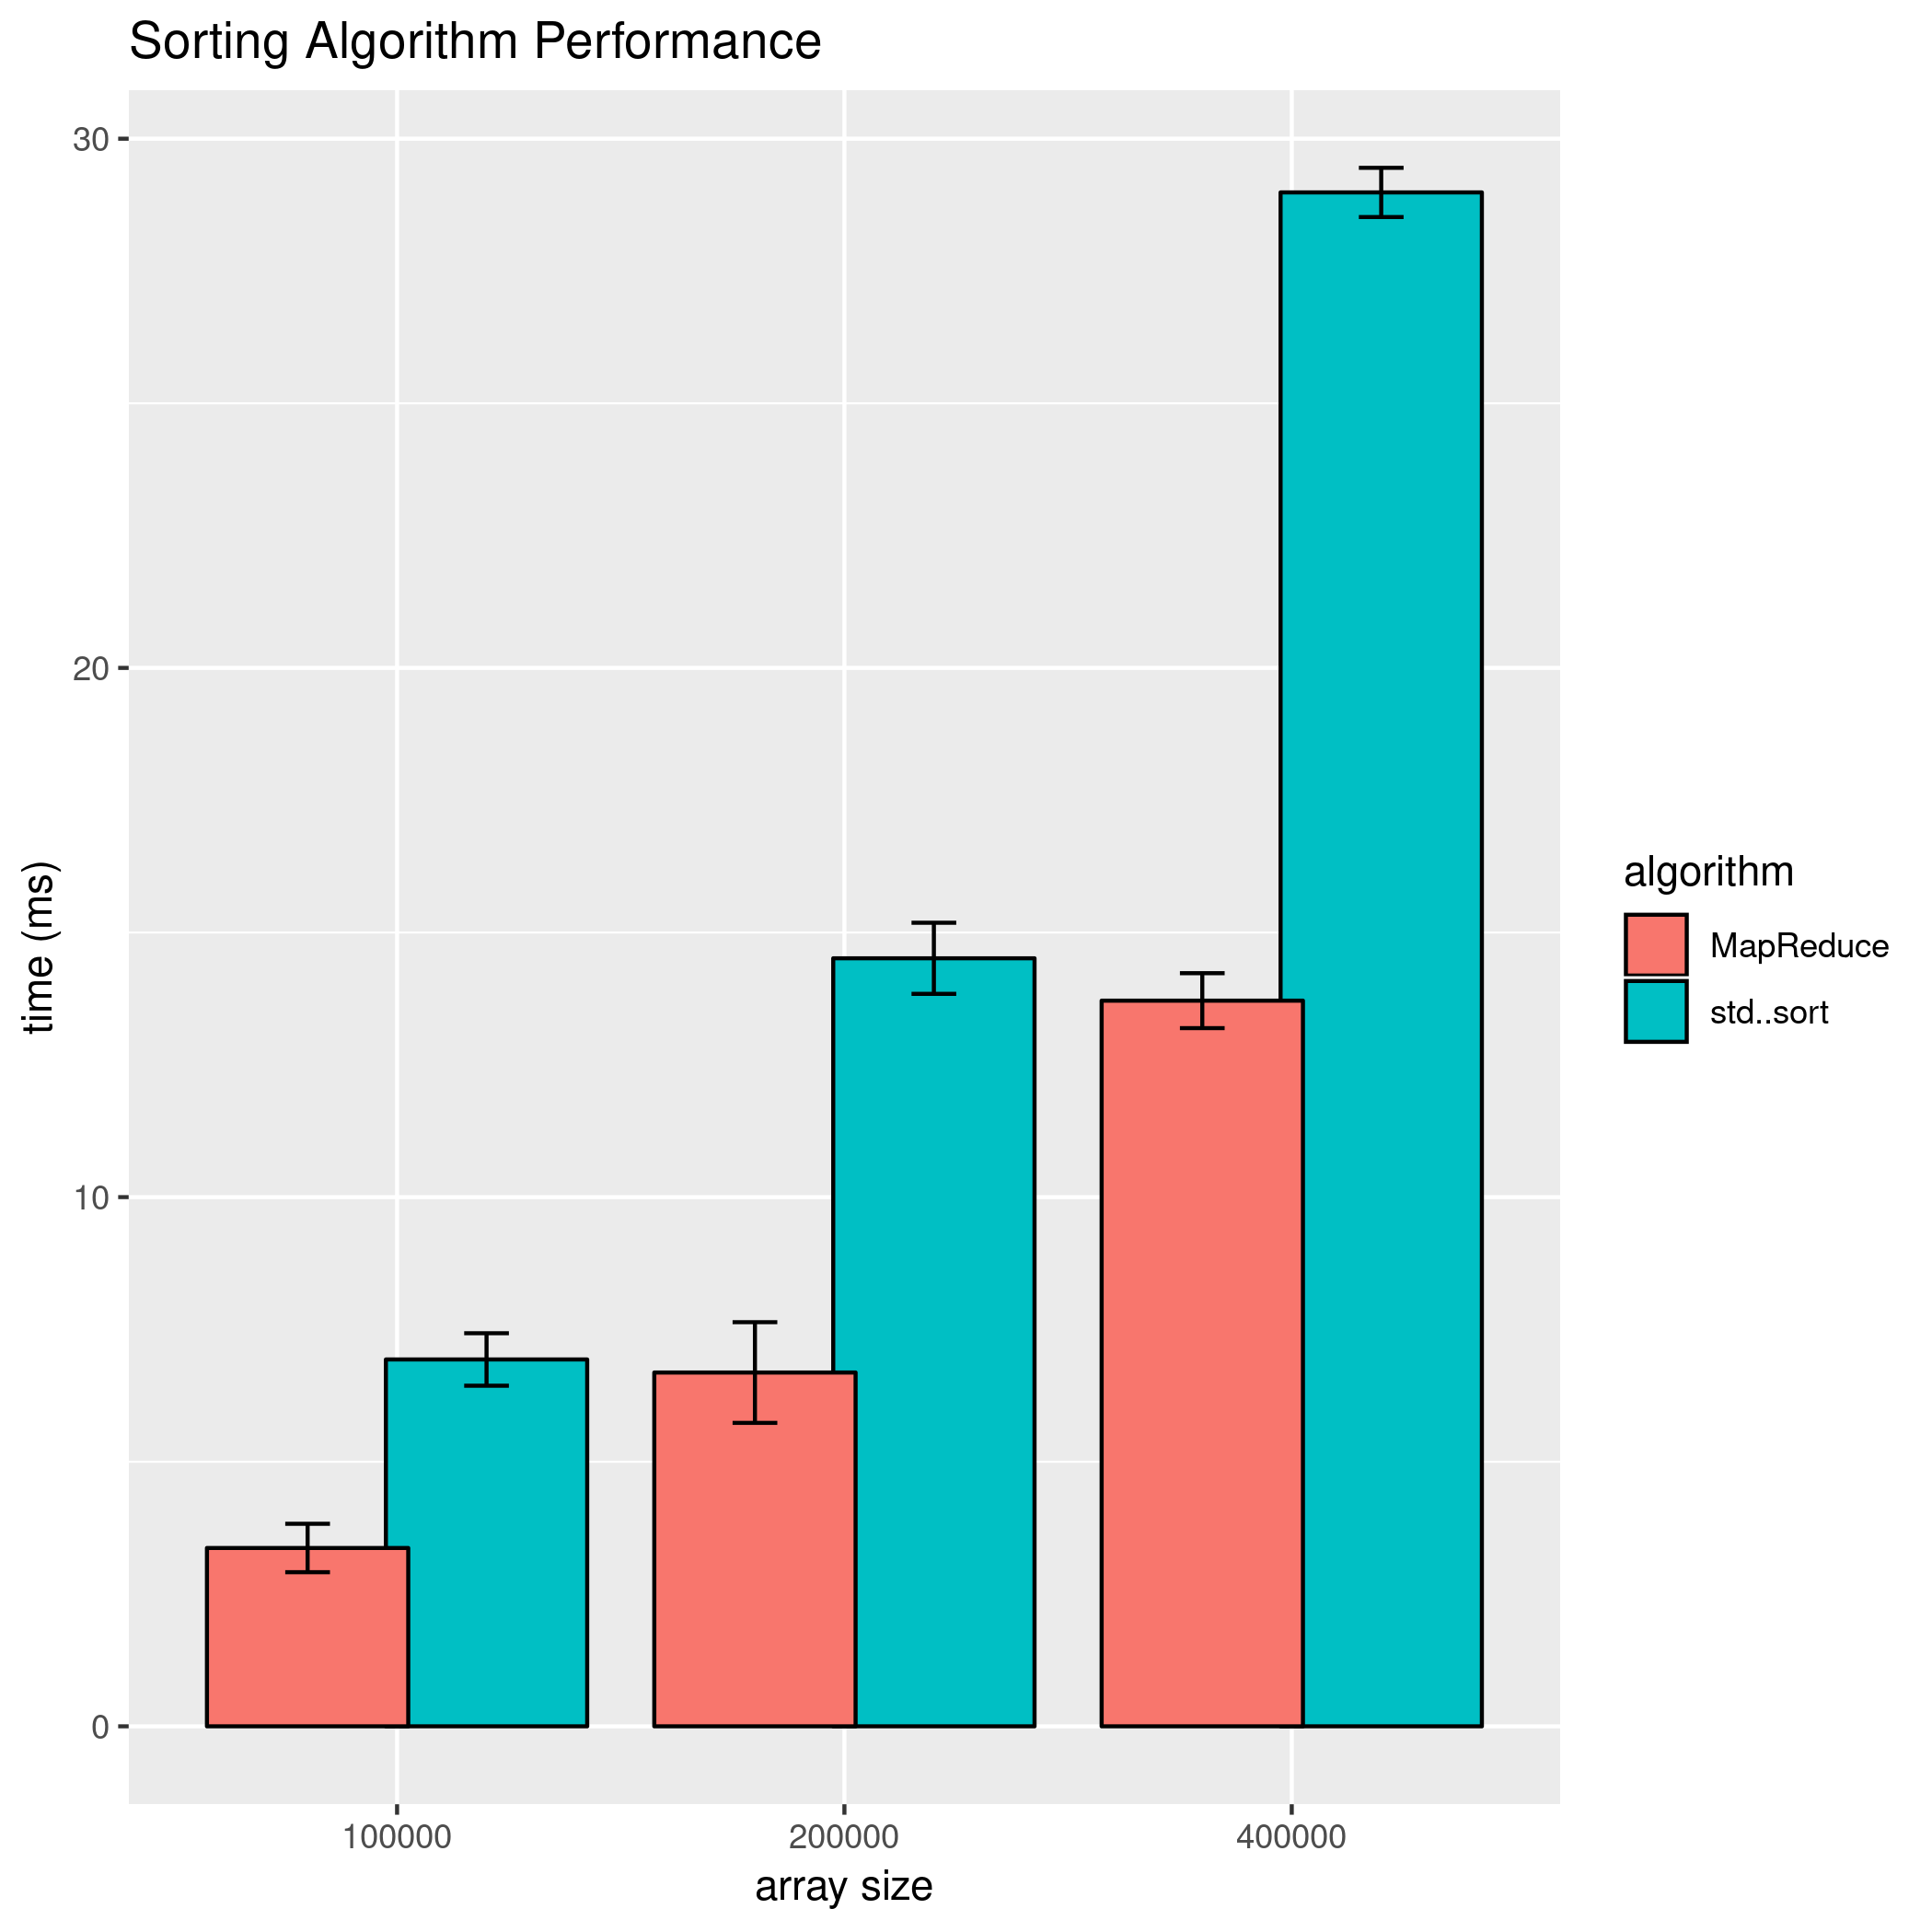
\includegraphics[width=0.75\textwidth]{sort-timing}
	\caption{MapReduce Sorting vs std::sort\label{fig:sort-timing}}
	\end{figure}

\subsection{Compared with Word Count}
	The main reason this algorithm is a better fit for MapReduce than word count is that it does much more of its work in the map and reduce stages, which are executed in parallel.
	We analyzed this behaviour in Callgrind and found that our MapReduce sorting algorithm does over 85\% of its computation in the map stage.
	A complete breakdown is shown in table~\ref{table:sortVwordcount}.

	\begin{table}[!h]\centering
	\renewcommand{\arraystretch}{1.3}
		\begin{tabular}{@{}lllll@{}}
			\toprule
			 & input stage & map stage & reduce stage & output stage\\ \midrule
			word count	&11.28\%	&11.72\%	&0.47\%	&11.21\%\\
			sort		&0.00\%		&85.71\%	&5.30\%	&4.76\%	\\
			\bottomrule
		\end{tabular}
		\caption{Word Count vs Sorting\label{table:sortVwordcount}}
	\end{table}


\section{Word count efficiency}
	Both implementations of the program counted the instances of unique words (including capitalization and adjacent punctuation marks) in \textit{Moby Dick; Or, The Whale} by Herman Melville, which is 2.1MB of text. They were run on the same machine with hardware to support twelve threads. Ten executions of each of the following implementations were conducted, with the duration and CPU usage measured with the built-in Linux \texttt{time} command:
	\begin{itemize}
	\item{single-threaded}
	\item{MapReduce, 4 threads}
	\item{MapReduce, 12 threads}
	\end{itemize}
	Additionally, call graphs for the single-threaded and MapReduce implementations were generated using Valgrind's Callgrind tool and visualized using KCachegrind.
\subsection{Single-threaded implementation}
	Table~\ref{table:singleImplWC} below shows the execution time, as well as CPU usage, for each of the ten single-threaded word count runs. The word count program ran for a mean user time of 0.0986 seconds and a mean system time of 0.1647 seconds, indicating that the processing time was dominated by the system calls associated with reading and writing the file.
	
	For a graphical representation of the call map for the single-threaded word count, see figure~\ref{fig:callMapSingleImpl} at the end of this document.
% single-threaded data - Moby Dick times
	\begin{table}[h]
	\centering
	\begin{tabular}{ccccc}
	\rowcolor[HTML]{FFFFC7} 
	\multicolumn{5}{c}{\cellcolor[HTML]{FFFFC7}\textbf{Execution times for single-threaded word count}} \\
	\rowcolor[HTML]{EFEFEF} 
	run \# & user (s) & system (s) & wall (s) & CPU usage (\%) \\
	1 & 0.106 & 0.160 & 0.860 & 30.2 \\
	2 & 0.097 & 0.161 & 0.860 & 29.0 \\
	3 & 0.098 & 0.161 & 0.860 & 29.0 \\
	4 & 0.084 & 0.181 & 0.860 & 30.2 \\
	5 & 0.099 & 0.162 & 0.860 & 29.0 \\
	6 & 0.091 & 0.167 & 0.860 & 29.0 \\
	7 & 0.114 & 0.154 & 0.860 & 30.2 \\
	8 & 0.093 & 0.168 & 0.720 & 34.7 \\
	9 & 0.108 & 0.164 & 0.860 & 30.2 \\
	10 & 0.096 & 0.169 & 0.860 & 29.0 \\
	\rowcolor[HTML]{D0F0D0} 
	\multicolumn{1}{r}{\cellcolor[HTML]{9AFF99}mean (s)} & 0.0986 & 0.1647 & 0.8460 & 30.05 \\
	\rowcolor[HTML]{ECF4FF} 
	\multicolumn{1}{r}{\cellcolor[HTML]{DAE8FC}std. dev. (s)} & 0.0088 & 0.0072 & 0.0443 & 1.739
	\end{tabular}
	\caption{Duration of single-threaded implementation measured by \texttt{time}\label{table:singleImplWC}}
	\end{table}
\subsection{MapReduce implementation}
	The MapReduce implementation of the word count was tested with four threads and then the full twelve threads the machine was capable of supporting.
	Tables~\ref{table:MR4ImplWC} and~\ref{table:MR12ImplWC} below show the execution time, as well as CPU usage, for each of the ten word counts run with MapReduce with four and twelve threads, respectively.
	Note that for a greater number of threads, the program actually took slightly longer to complete.
	Further, as the thread count increased, the CPU usage also increased, going from an average of 43.87\% with four threads to an average of 55.13\% with 12 threads.

	The four- and twelve-threaded MapReduce implementation timings both showed a greater user time compared to system time, on average.
	With four threads, the mean user time was 222 milliseconds and the mean system time was 198 milliseconds.
	With twelve threads, the mean user time was 311 milliseconds and the mean system time was 229 milliseconds.
	This meant most of the time was spent in the program rather than system calls, as was the case with single-threading.
	However, both system \textit{and} user time were greater in the MapReduce implementation than the single-threaded implementation.

	For a graphical representation of the call map for the MapReduce word count, see figure~\ref{fig:callMapMRImpl} at the end of this document.
% MapReduce data (4 threads) - Moby Dick times
	\begin{table}[h]
	\centering
	\begin{tabular}{ccccc}
	\multicolumn{5}{c}{\cellcolor[HTML]{FFFFC7}\textbf{Execution times for MapReduce word count - 4 threads}} \\
	\cellcolor[HTML]{EFEFEF}run \# & \cellcolor[HTML]{EFEFEF}user (s) & \cellcolor[HTML]{EFEFEF}system (s) & 				\cellcolor[HTML]{EFEFEF}wall (s) & \cellcolor[HTML]{EFEFEF}CPU usage (\%) \\
	1 & 0.206 & 0.215 & 0.93 & 44.0 \\
	2 & 0.225 & 0.213 & 0.95 & 45.2 \\
	3 & 0.231 & 0.178 & 0.99 & 40.4 \\
	4 & 0.236 & 0.187 & 0.94 & 43.6 \\
	5 & 0.211 & 0.211 & 0.94 & 44.6 \\
	6 & 0.215 & 0.203 & 0.96 & 42.7 \\
	7 & 0.231 & 0.195 & 0.95 & 44.2 \\
	8 & 0.212 & 0.200 & 0.99 & 41.4 \\
	9 & 0.210 & 0.210 & 0.81 & 51.8 \\
	10 & 0.243 & 0.167 & 0.98 & 40.8 \\
	\rowcolor[HTML]{D0F0D0} 
	\multicolumn{1}{r}{\cellcolor[HTML]{9AFF99}mean (s)} & 0.2220 & 0.1979 & 0.9440 & 43.87 \\
	\rowcolor[HTML]{ECF4FF} 
	\multicolumn{1}{r}{\cellcolor[HTML]{DAE8FC}std. dev. (s)} & 0.0128 & 0.0161 & 0.0517 & 3.237
	\end{tabular}
	\caption{Duration of MapReduce implementation measured by \texttt{time}, with four threads\label{table:MR4ImplWC}}
	\end{table}
% MapReduce data (12 threads) - Moby Dick times
	\begin{table}[h]
	\centering
	\begin{tabular}{ccccc}
	\multicolumn{5}{c}{\cellcolor[HTML]{FFFFC7}\textbf{Execution times for MapReduce word count - 12 threads}} \\
	\rowcolor[HTML]{EFEFEF} 
	run \# & user (s) & system (s) & wall (s) & CPU usage (\%) \\
	1 & 0.305 & 0.232 & 1.02 & 51.9 \\
	2 & 0.277 & 0.255 & 0.94 & 55.3 \\
	3 & 0.348 & 0.213 & 0.95 & 57.8 \\
	4 & 0.347 & 0.206 & 0.97 & 55.6 \\
	5 & 0.331 & 0.198 & 0.94 & 55.3 \\
	6 & 0.310 & 0.219 & 0.96 & 54.1 \\
	7 & 0.293 & 0.238 & 0.98 & 53.0 \\
	8 & 0.302 & 0.239 & 0.96 & 55.2 \\
	9 & 0.265 & 0.274 & 0.94 & 56.3 \\
	10 & 0.331 & 0.213 & 0.95 & 56.8 \\
	\rowcolor[HTML]{D0F0D0} 
	\multicolumn{1}{r}{\cellcolor[HTML]{9AFF99}mean (s)} & 0.3109 & 0.2287 & 0.9610 & 55.13 \\
	\rowcolor[HTML]{ECF4FF} 
	\multicolumn{1}{r}{\cellcolor[HTML]{DAE8FC}std. dev. (s)} & 0.0282 & 0.0236 & 0.0247 & 1.751
	\end{tabular}
	\caption{Duration of MapReduce implementation measured by \texttt{time}, with twelve threads\label{table:MR12ImplWC}}
	\end{table}
\subsection{Comparison}
	An increase in threads used in the implementation of word counts appears to correspond with higher overall CPU usage, processing time, and wall time.
	This indicates that for the word count problem, MapReduce succeeds only in making more work for itself, while failing to reap any of the potential benefits of parallelism.
	The single-threaded implementation came in with a mean wall time of 0.8460 seconds, the four-threaded MapReduce implementation with a mean wall time of 0.9440 seconds, and the twelve-threaded MapReduce implementation with a mean wall time of 0.9610 seconds.
	
\section{Alternate Workload}
In addition to the sort program, a matrix multiplication algorithm was also adapted to the MapReduce interface. The algorithm is described in detail in the blog post “Matrix Multiplication with MapReduce”\footnote{https://lendap.wordpress.com/2015/02/16/matrix-multiplication-with-mapreduce/}

The algorithm is intended for multiplying very large, sparse matrices (hundreds of thousands or millions of rows and columns) and distributing the task over many machines. Because of the permutative nature of matrix multiplication this requires significant duplication of data. The mapper stage copies every element of A for every column in B and every element in B for every row in A. MapReduce makes this copying necessary because each worker in the reduce stage has access only to its individual piece of the data. 

On a single machine, in a multi-threaded context, the MapReduce matrix multiplication operation took ~100 times as long as the implementation found in the NumPy numerical computation package for Python, for a 100x100 matrix. Naturally, it also consumed significantly more memory. 

In a distributed system, the workers cannot share memory, so the copying done by the MapReduce method is likely a lower bound on the amount of copying necessary for any distributed method. Since the workers are responsible for the copying, each value only needs to be transmitted once in the input stage. 

	
\section{Most appropriate workload for MapReduce}
Our investigation confirmed that MapReduce is most suitable for applications where:
\begin{itemize}
\item The input data can be partitioned into discrete pieces which can be operated on in isolation. 
\item The computation required for each piece is significant enough to overcome the overhead of partitioning, distributing and then recombining the data. 
\end{itemize}
	
\section{Impact of using multiple machines on execution speed}
The primary difference between a multi-machine implementation and a local, multi-threaded implementation is that the overhead of moving data during the input, shuffle, and output stages is much higher when moving data between machines, versus merely moving data around in local memory. This increases the importance of the suitability criteria described above. 

\newpage
	\begin{figure}[h]
	\centering
	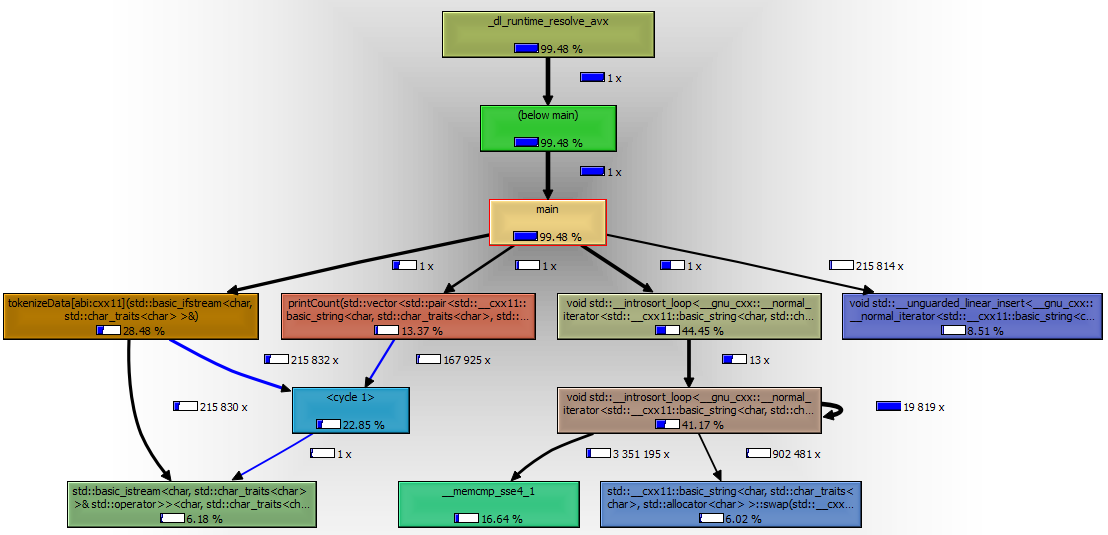
\includegraphics[width=1.35\textwidth, angle=90]{call-graph-part3-final-cropped}
	\caption{Call map for single-threaded implementation of word count\label{fig:callMapSingleImpl}}
	\end{figure}
\newpage
	\begin{figure}[h]
	\centering
	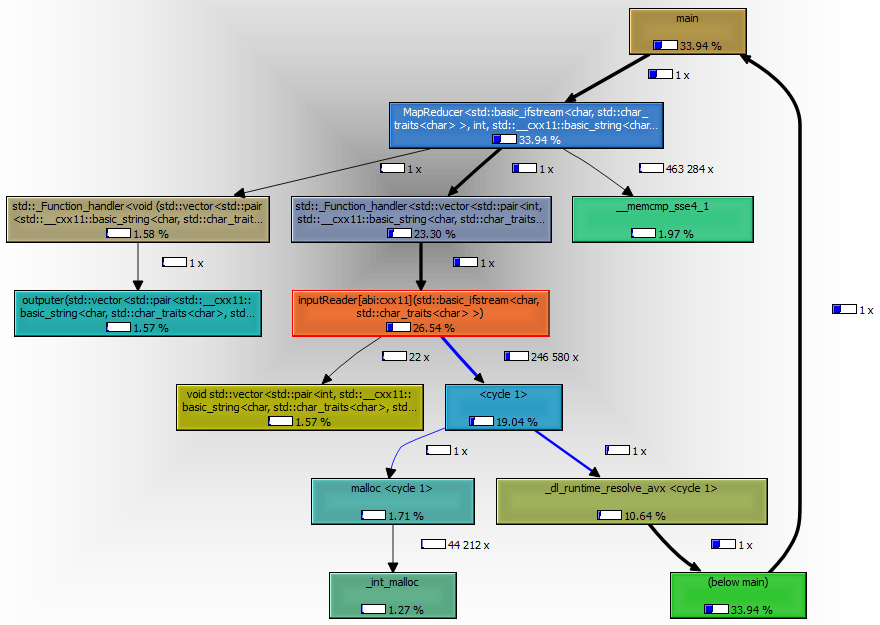
\includegraphics[width=1.35\textwidth, angle=90]{call-graph-part4-final-cropped}
	\caption{Call map for MapReduce implementation of word count (twelve threads)\label{fig:callMapMRImpl}}
	\end{figure}
\end{document}
